\documentclass[10pt,xcolor=dvipsnames]{beamer}

% \usepackage{arev}
% \usepackage{sourcesanspro}
% \usepackage{sourcecodepro}

\usepackage{fontspec}
\setsansfont{DejaVu Sans}
%\setmonofont{Input Mono Narrow}
\setmonofont{Hack}

\usepackage[utf8]{inputenc}
\usepackage[english]{babel}
\usepackage{listings}
\usepackage{graphicx}
\usepackage{epstopdf}

\setbeamertemplate{navigation symbols}{}
\setbeamertemplate{footline}[frame number]{}
\setbeamercolor{frametitle}{fg=Black,bg=White}
%\setbeamertemplate{footline}{\hfill\insertframenumber~\vrule~\inserttotalframenumber}
\lstset{
  stepnumber=1,
  breaklines=true,
  basicstyle=\ttfamily\scriptsize,
  numberstyle=\tiny,
  commentstyle=\color{gray},
  showstringspaces=false,
  keepspaces=true
}

\renewcommand\big[1]{
  \begin{center}
    \Large{#1}
  \end{center}
}

\begin{document}

\begin{frame}
  \centering\Huge{Data-Oriented Design}
\end{frame}

\begin{frame}
  \centering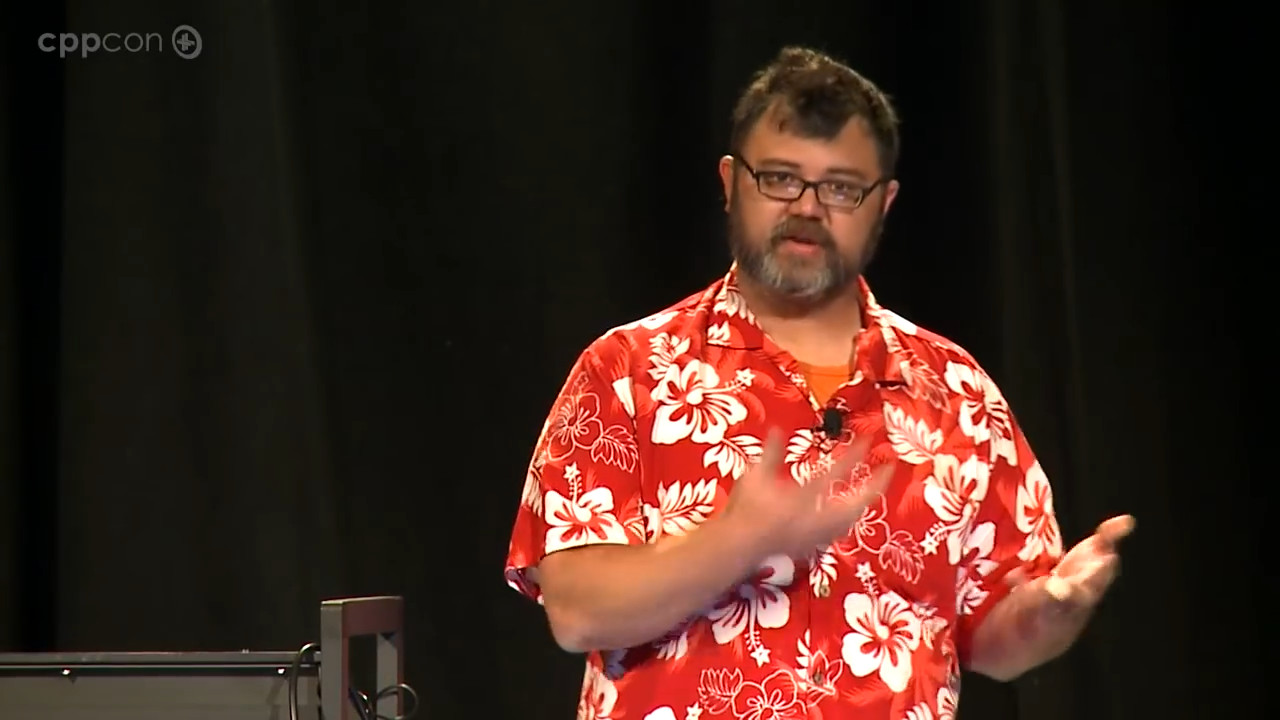
\includegraphics[scale=0.2]{mike-acton.jpg}
  \vskip 0.5cm
  Mike Acton, \textsl{Data-Oriented Design and C++}, CppCon 2014
\end{frame}

% \begin{frame}
%   \big{The Three Lies (According to Mike Acton)}
%   \begin{itemize}
%     \item Software is a platform
%     \item Code is more important than data
%     \item Code designed around model of the world
%   \end{itemize}
% \end{frame}

% \begin{frame}
%   \big{Mike Acton Made Me Feel Uncomfortable}
%   He was basically saying that I was coding wrong, and had been coding wrong for \emph{years}.
%   \begin{itemize}
%     \item I thought about \emph{the code} too much
%     \item I thought about \emph{the data} not enough
%     \item I didn't take the hardware in consideration
%   \end{itemize}
%   \vskip .5cm
%   Conclusion: ``Clearly this Mike Acton guy doesn't know anything and I will ignore him forever!''
% \end{frame}

\begin{frame}
  \big{TLDR}
  \vskip 1cm
  \centering
  In FP/OOP, you focus on organizing your \emph{code}.
  \vskip .5cm
  In DOD, you focus on organizing your \emph{data}.
\end{frame}

\begin{frame}
  \big{The ``Why'' of Data-Oriented}
\end{frame}

\begin{frame}{The Problem}
  \begin{quote}
    Picture this: Toward the end of the development cycle, your game
    crawls, but you don’t see any obvious hotspots in the profiler.
    The culprit? \textbf{Random memory access patterns and constant
      cache misses.} In an attempt to improve performance, you try to
    parallelize parts of the code, but it takes heroic efforts, and,
    in the end, you barely get much of a speed-up due to all the
    synchronization you had to add. To top it off, the code is so
    complex that fixing bugs creates more problems, and the thought of
    adding new features is discarded right away. Sound familiar?
  \end{quote}

  ---Noel Llopis, \textsl{Data-Oriented Design (Or Why You Might Be Shooting Yourself in The Foot With OOP)}
\end{frame}

\begin{frame}{The Problem}
  \begin{quote}
    That scenario pretty accurately describes almost every game I’ve
    been involved with for the last 10 years. The reasons aren’t the
    programming languages we’re using, nor the development tools, nor
    even a lack of discipline. In my experience, \textbf{it’s object-oriented
    programming (OOP) and the culture that surrounds it that is in
    large part to blame} for those problems. OOP could be hindering
    your project rather than helping it!
  \end{quote}

  ---Noel Llopis, \textsl{Data-Oriented Design (Or Why You Might Be Shooting Yourself in The Foot With OOP)}
\end{frame}

\begin{frame}{The Problem}{Summary}
  \begin{itemize}
    \item Game runs too slowly
    \item Why? Too many cache misses
    \item Why? Random---rather than sequential and predictable---accesses to memory
    \item Why? Common OO usage allocates objects in a tree/graph independent of the memory hierarchy
  \end{itemize}
\end{frame}

\begin{frame}
  \big{The problem with OO culture}
\end{frame}

\begin{frame}{Micro-example}
  An example of common OO design advice.
  \vskip .5cm
  \begin{quote}
    Depend on abstractions, not on concretions\footnote{BTW: Concretion is a geological term; it's not the opposite of abstraction.}.
  \end{quote}
  \vskip .5cm
  \small{Uncle Bob}

\end{frame}

\begin{frame}[fragile]{Micro-example}
  \begin{lstlisting}[language=Java]
    static private double arrayAvg(double[] it) {
        double sum = 0.0;
        for (double x: it) {
            sum += x;
        }
        return sum / it.length;
    }

    /* VERSUS */

    static private double iteratorAvg(Iterator<Double> it) {
        double sum = 0.0;
        int len = 0;
        while (it.hasNext()) {
            sum += it.next();
            len += 1;
        }
        return sum / len;
    }
  \end{lstlisting}
\end{frame}

\begin{frame}[fragile]{Micro-example}
  \begin{center}
    \begin{tabular}{l | r}
      Method         & Time \\
      \hline
      Array          & 0.6 sec \\
      Iterator       & 1.2 sec
    \end{tabular}
  \end{center}
  \begin{itemize}
    \item The ``good OO'' implementation is twice as slow
    \item The array version can be optimized (SIMD, split array + spawn threads)
    \item The interface version cannot be optimized.
    \item What happens in a system where \emph{everything} follows this advice?
  \end{itemize}
\end{frame}

\begin{frame}{Micro-example}
  \begin{quote}
    Different problems require different solutions.
    \vskip .5cm
    Solving problems you probably don't have creates more problems you
    definitely do have.
  \end{quote}
  \vskip .5cm
  \small{Mike Acton}
\end{frame}

\begin{frame}
  \big{The ``What'' of Data-Oriented}
\end{frame}

\begin{frame}[t]{What is data-oriented design?}
  \vskip 2cm
  \begin{quote}
    Data-oriented design is an approach to optimising programs by
    carefully considering the memory layout of data structures
  \end{quote}
  \vskip .5cm
  \small{James McMurray, \textsl{An introduction to Data Oriented Design with Rust}}
\end{frame}

\begin{frame}[t]{What is data-oriented design?}
  \vskip 2cm
  \begin{quote}
    Data-oriented design is an approach to \textbf{organizing}
    programs by carefully considering the memory layout of data
    structures
  \end{quote}
\end{frame}

\begin{frame}{What is data-oriented design?}
  \centering\emph{Carefully considering the memory layout of data}
\end{frame}


\begin{frame}{What is data-oriented design?}
  \centering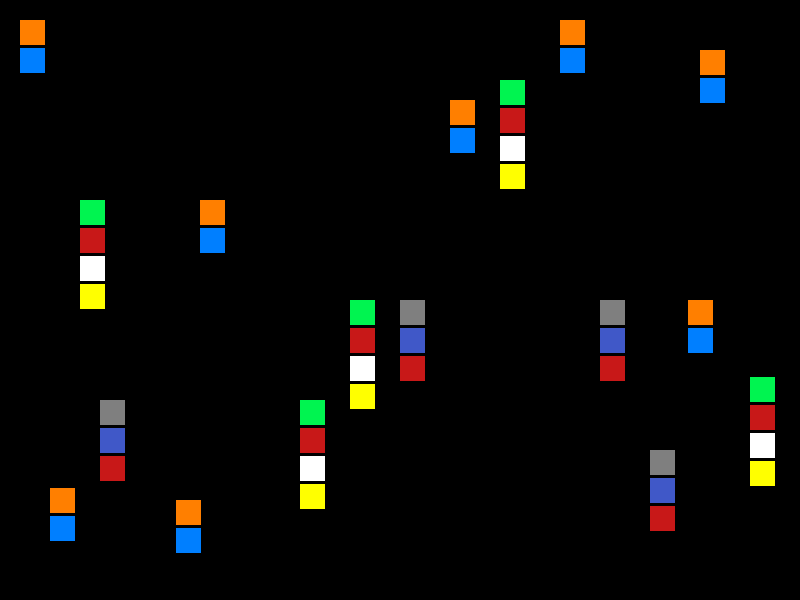
\includegraphics[scale=0.75]{oo-layout.png}
\end{frame}

\begin{frame}{What is data-oriented design?}
  \centering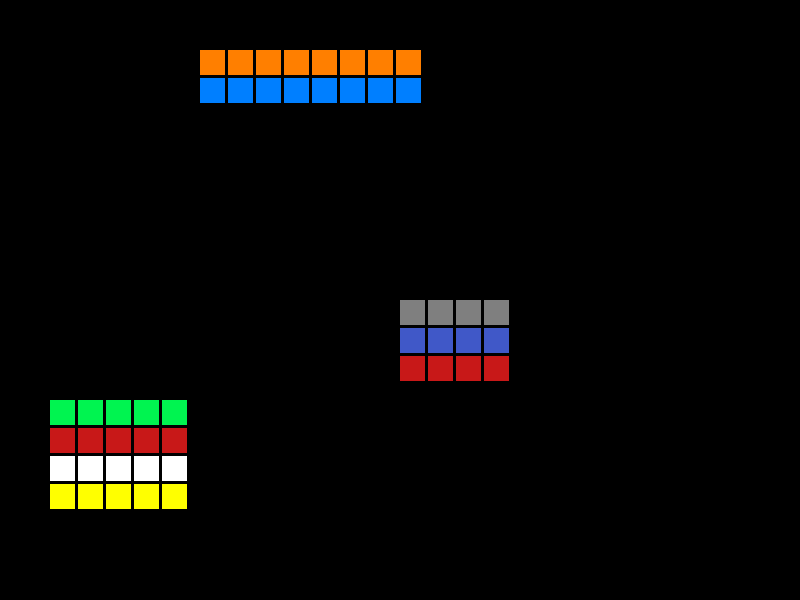
\includegraphics[scale=0.75]{do-layout.png}
\end{frame}


% \begin{frame}{What is data-oriented programming?}
%   \begin{itemize}
%     \item What hardware am I targeting?
%     \item What OS am I targeting?
%     \item What operations need to be the fastest?
%     \item How large is my data?
%     \item Is my data read-only or read-write?
%     \item Is my data sorted?
%     \item What's the distribution of values?
%   \end{itemize}
% \end{frame}

% \begin{frame}{What is data-oriented programming?}
%   \begin{itemize}
%     \item Data is more important than code
%     \item Your job is \emph{not} to write code
%     \item Your job is to transform data
%     \item Code is the tool you use to do your job
%   \end{itemize}
% \end{frame}

\begin{frame}{Computer Memory in Modern Times}
  \centering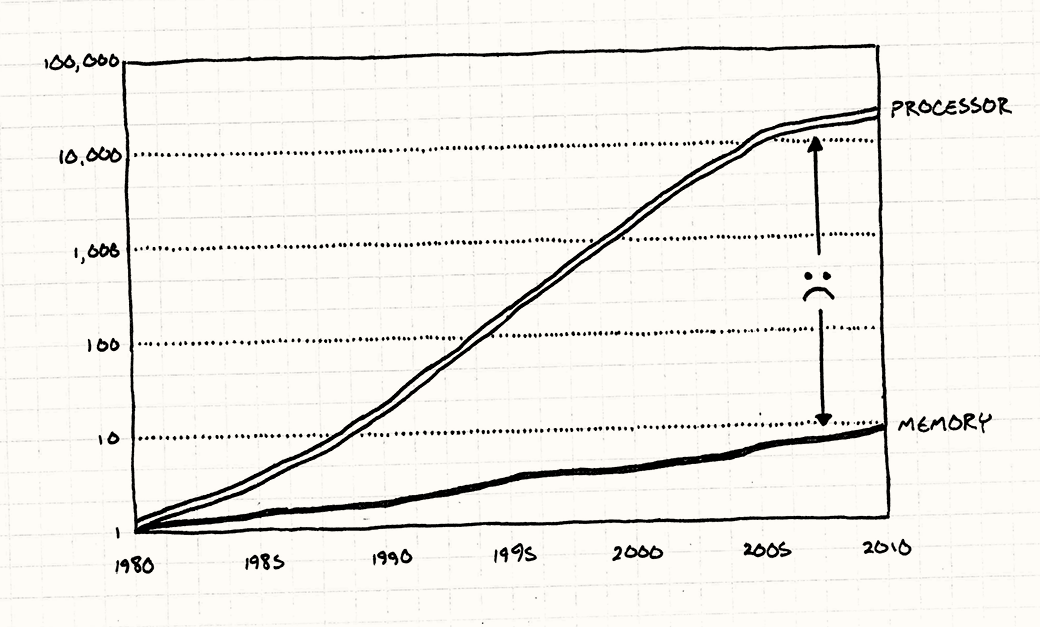
\includegraphics[scale=0.3]{data-locality-chart.png}
  \tiny{Source: \url{http://gameprogrammingpatterns.com/data-locality.html}}
\end{frame}

\begin{frame}{Computer Memory in Modern Times}
  \centering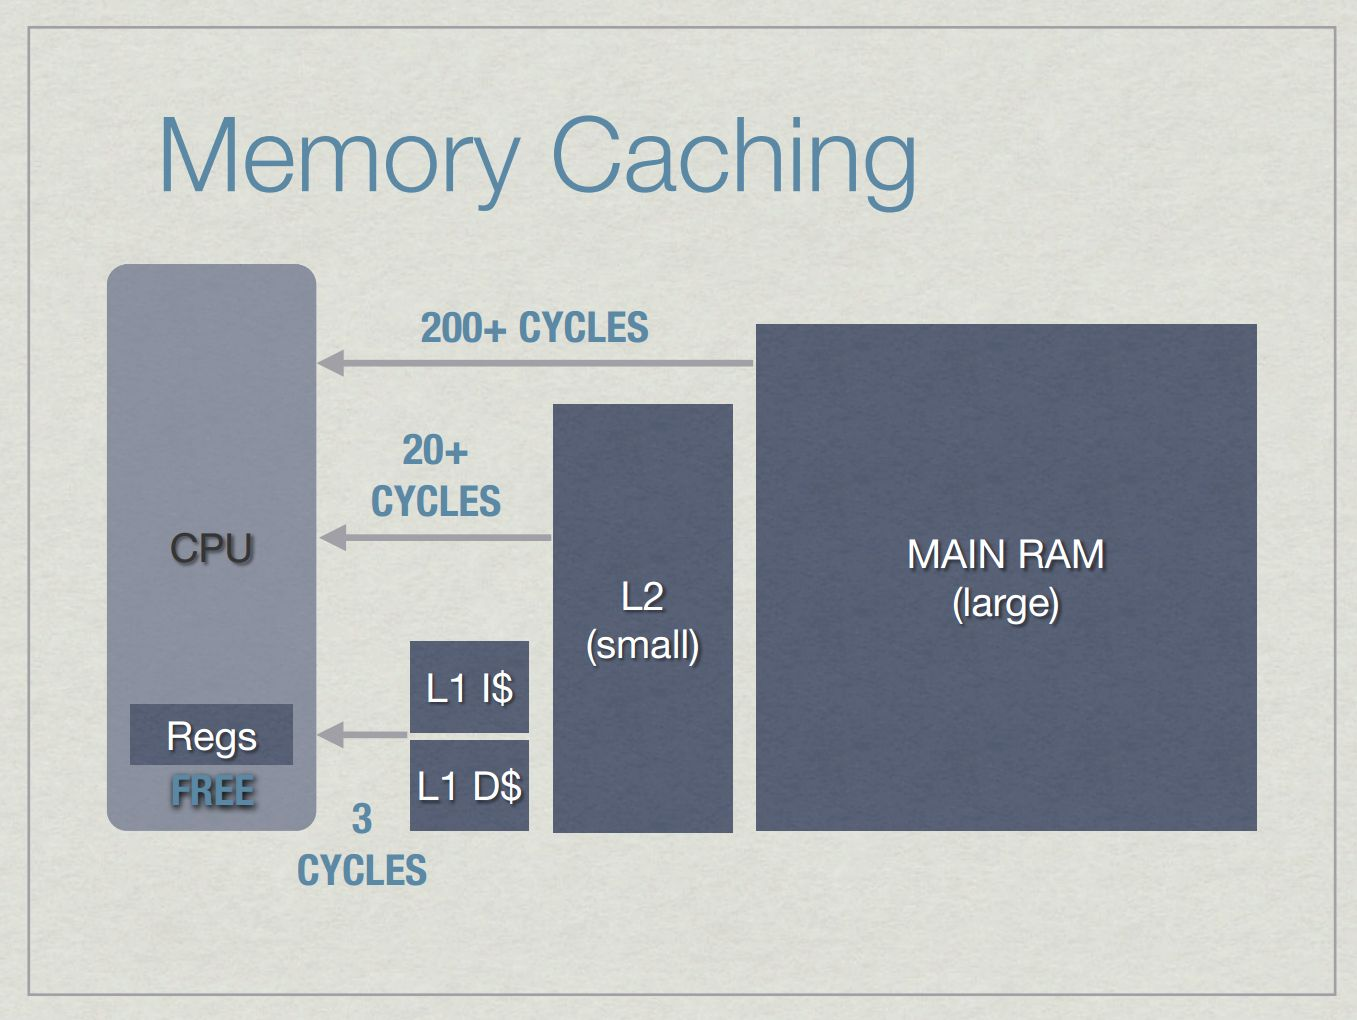
\includegraphics[scale=0.2]{memory-hierarchy.jpg}

  \tiny{Source: Jason Gregory, \textsl{Game Engine Architecture}}
\end{frame}

\begin{frame}{Computer Memory in Modern Times}
  \big{Demo}
  \centering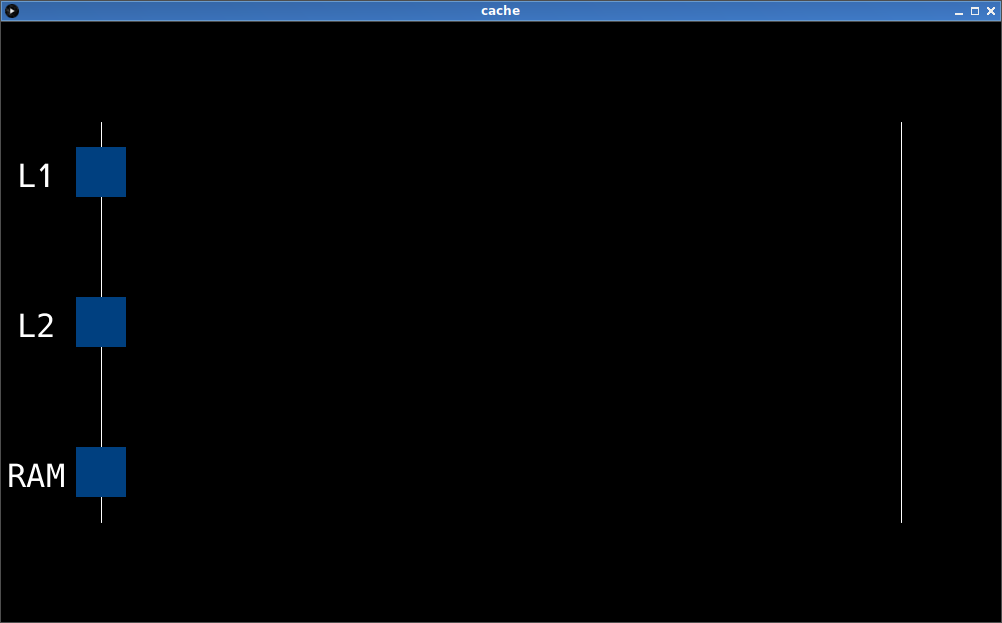
\includegraphics[scale=0.5]{cache-demo.png}
\end{frame}

\begin{frame}
  \big{The ``How'' of Data-Oriented}
\end{frame}

\begin{frame}
  \big{Better cache use example}
\end{frame}

\begin{frame}{Cache example}
  \big{Find the user that logged in most recently}
\end{frame}

\begin{frame}[fragile]{The input file}
  \begin{lstlisting}
0:alicea_brittnee:/home/alicea_brittnee:/bin/bash:1576347215
1:carolee_ange:/home/carolee_ange:/bin/bash:1572506918
2:claudie_halsted:/home/claudie_halsted:/bin/bash:1576263841
3:brianne_hizar:/home/brianne_hizar:/bin/bash:1576619633
4:marika_barraza:/home/marika_barraza:/bin/bash:1566035342
5:cristiona_randolf:/home/cristiona_randolf:/bin/bash:1573717947
6:meghan_lief:/home/meghan_lief:/bin/bash:1572370708
7:elly_lemmuela:/home/elly_lemmuela:/bin/bash:1590743916
8:rora_baily:/home/rora_baily:/bin/bash:1567493247
9:sharron_medor:/home/sharron_medor:/bin/bash:1573733695
...
  \end{lstlisting}
\end{frame}

\begin{frame}[fragile]{Cache example}{Array of Structs ($\sim$ Postgresql)}
  \begin{lstlisting}[language = Go]
type User = struct {
        id         int64
        username   string
        homedir    string
        shell      string
        last_login int64
}


latest_timestamp := int64(0)
latest_username := ""
for _, user := range users {
        if user.last_login > latest_timestamp {
                latest_timestamp = user.last_login
                latest_username = user.username
        }
}
\end{lstlisting}
\end{frame}

\begin{frame}[fragile]{Cache example}{Array of Structs}
  \begin{lstlisting}
:) for _ in {1..5}; do go run most_recent_login.go; done
last_login: 1596901628; user: eolanda_pinchas, time: 8.43612ms
last_login: 1596901628; user: eolanda_pinchas, time: 11.060461ms
last_login: 1596901628; user: eolanda_pinchas, time: 11.229049ms
last_login: 1596901628; user: eolanda_pinchas, time: 8.513542ms
last_login: 1596901628; user: eolanda_pinchas, time: 8.479247ms
\end{lstlisting}
\vskip 1.5cm
\centering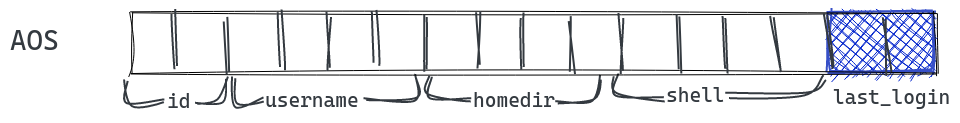
\includegraphics[scale=0.3]{aos.png}
\end{frame}

\begin{frame}[fragile]{Cache example}{Hot/Cold Split}
  \begin{lstlisting}[language = Go]
type UserInfo = struct {
        id       int64
        username string
        homedir  string
        shell    string
}
type User = struct {
        info       *UserInfo
        last_login int64
}


latest_timestamp := int64(0)
latest_username := ""
for _, user := range users {
        if user.last_login > latest_timestamp {
                latest_timestamp = user.last_login
                latest_username = user.info.username
        }
}
  \end{lstlisting}
\end{frame}

\begin{frame}[fragile]{Cache example}{Hot/Cold Split}
  \begin{lstlisting}
:) for _ in {1..5}; do go run most_recent_login.go; done
last_login: 1596901628; user: eolanda_pinchas; time: 2.549558ms
last_login: 1596901628; user: eolanda_pinchas; time: 2.53031ms
last_login: 1596901628; user: eolanda_pinchas; time: 2.588776ms
last_login: 1596901628; user: eolanda_pinchas; time: 2.536942ms
last_login: 1596901628; user: eolanda_pinchas; time: 2.549696ms
\end{lstlisting}
\vskip 1.5cm
\centering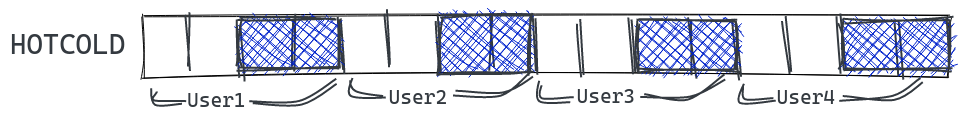
\includegraphics[scale=0.3]{hotcold.png}
\end{frame}

\begin{frame}[fragile]{Cache example}{Struct of Arrays ($\sim$ Vertica)}
  \begin{lstlisting}[language = Go]
type Users = struct {
        id         []int64
        username   []string
        homedir    []string
        shell      []string
        last_login []int64
}


latest_timestamp := int64(0)
latest_entity := 0
for i, last_login := range users.last_login {
        if last_login > latest_timestamp {
                latest_timestamp = last_login
                latest_entity = i
        }
}
\end{lstlisting}
\end{frame}

\begin{frame}[fragile]{Cache example}{Struct of Arrays}
  \begin{lstlisting}
:) for _ in {1..5}; do go run most_recent_login.go; done
last_login: 1596901628; user: eolanda_pinchas; time: 1.45387ms
last_login: 1596901628; user: eolanda_pinchas; time: 1.449812ms
last_login: 1596901628; user: eolanda_pinchas; time: 1.464322ms
last_login: 1596901628; user: eolanda_pinchas; time: 1.460788ms
last_login: 1596901628; user: eolanda_pinchas; time: 1.446045ms
\end{lstlisting}
\vskip 1.5cm
\centering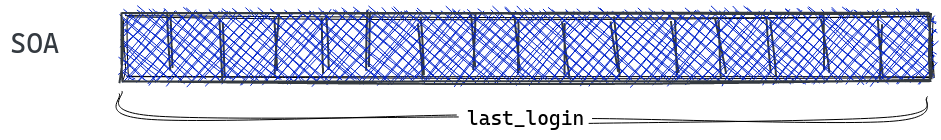
\includegraphics[scale=0.3]{soa.png}
\end{frame}

\begin{frame}{Cache example}{Takeaways}
  \begin{itemize}
    \item Same complexity ($O(n)$), but in practice constants \emph{do} matter
    \item By considering the layout of data, we got a 6x speed-up
    \item \emph{We} made the program 6x faster, not the compiler
  \end{itemize}
\end{frame}

\begin{frame}
  \big{An example that has nothing to do with cache}
\end{frame}

\begin{frame}[t,fragile]{An example that has nothing to do with cache}{The Problem}
  \big{segvault-client}

  Richard found that a lot of time in rtb-gateway was spent calling the function \texttt{setelement}

  \vskip 1cm
  \begin{lstlisting}
FUNCTION                        CALLS        %
--------                        -----  -------
...
cowboy_handler:execute/2          146     5.01
segvault_protocol:collect/2    129136     7.72
erlang:setelement/3            143367    10.49
  \end{lstlisting}
\end{frame}

\begin{frame}[t,fragile]{An example that has nothing to do with cache}{The Problem}
  \begin{lstlisting}
collect([Seg|More], #segvault_response {
  lotame = Lotame,
  adobe = Adobe, ...} = Acc) ->
  {SegmentType, SegmentId} = {
    decode_segment_type(Seg bsr ?SEGMENT_BITS),
    Seg band ?SEGMENT_MASK
  },
  Acc2 = case SegmentType of
    lotame ->
      Acc#segvault_response { lotame = [SegmentId | Lotame] };
    adobe ->
      Acc#segvault_response { adobe = [SegmentId | Adobe] };
    \end{lstlisting}
    For those who don't read Erlang:
    \begin{itemize}
      \item We process one segment at a time
      \item We cons the segment to the appropriate list
      \item We setelement the new list in the response
    \end{itemize}
\end{frame}

\begin{frame}[fragile]{An example that has nothing to do with cache}{The Data}
  \begin{lstlisting}
    ADOBE:11111
    ADOBE:11112
    LOTAME:22221
    LOTAME:22222
    LOTAME:22223
    LOTAME:22224
    LIVERAMP3P:33331
    LIVERAMP3P:33332
    LIVERAMP3P:33333
    ...
  \end{lstlisting}
  \vskip 1cm
  Holy fish! The segments are grouped by segment type!
\end{frame}

\begin{frame}[fragile]{An example that has nothing to do with cache}{The Solution}
  \begin{itemize}
    \item Accumulate segments in a list (one cons per segment)
    \item When the segment type changes, store list in accumulator, empty list (one setelement per \emph{segment type})
  \end{itemize}
\end{frame}

\begin{frame}{An example that has nothing to do with cache}{The Result}
  \centering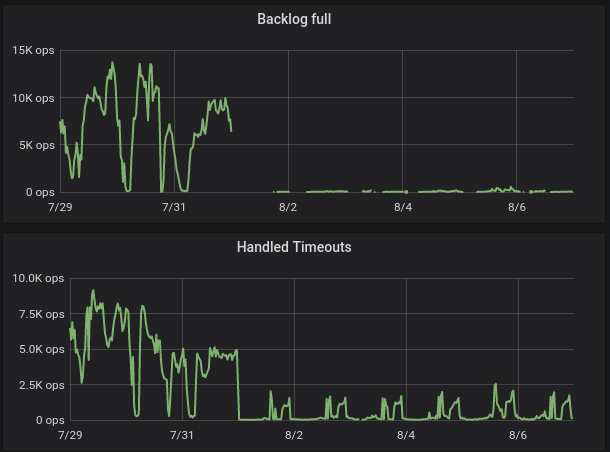
\includegraphics[scale=1.8]{grafana.png}
\end{frame}

\begin{frame}
  \centering\Huge{Extra slides}
\end{frame}

\begin{frame}
  \big{Random wisdom from Mike Acton}
\end{frame}

\begin{frame}
  \begin{quote}
    The purpose of all programs, and all parts of those programs, is
    to transform data from one form to another.
  \end{quote}
\end{frame}

\begin{frame}
  \begin{quote}
    If you don't understand the data you don't understand the problem.
    \vskip .5cm
    Conversly, understand the problem by understanding the data.
  \end{quote}
\end{frame}

\begin{frame}
  \begin{quote}
    Different problems require different solutions.
    \vskip .5cm
    If you have different data, you have a different problem.
  \end{quote}
\end{frame}

\begin{frame}
  \begin{quote}
    Where there is one there are many.
  \end{quote}
\end{frame}

\begin{frame}
  \begin{quote}
    The more context you have, the better you can make the solution.
  \end{quote}
\end{frame}

\begin{frame}
  \begin{quote}
    There is no ideal, abstraction solution to the problem.
    \vskip .5cm
    You can't ``future proof''
  \end{quote}
\end{frame}

\begin{frame}
  \begin{quote}
    Solve the most common case first, not the most generic.
  \end{quote}
\end{frame}

\begin{frame}{Computer Memory in Modern Times}
  \big{2-minute cache course}
  \begin{itemize}
    \item If a memory address is cached, don't go to memory
    \item When fetching from memory, bring an entire cache line (64~bytes) into the cache
    \item Best way to take advantage of the cache: keep data contiguous in memory
  \end{itemize}
\end{frame}

\begin{frame}{Computer Memory in Modern Times}
  \centering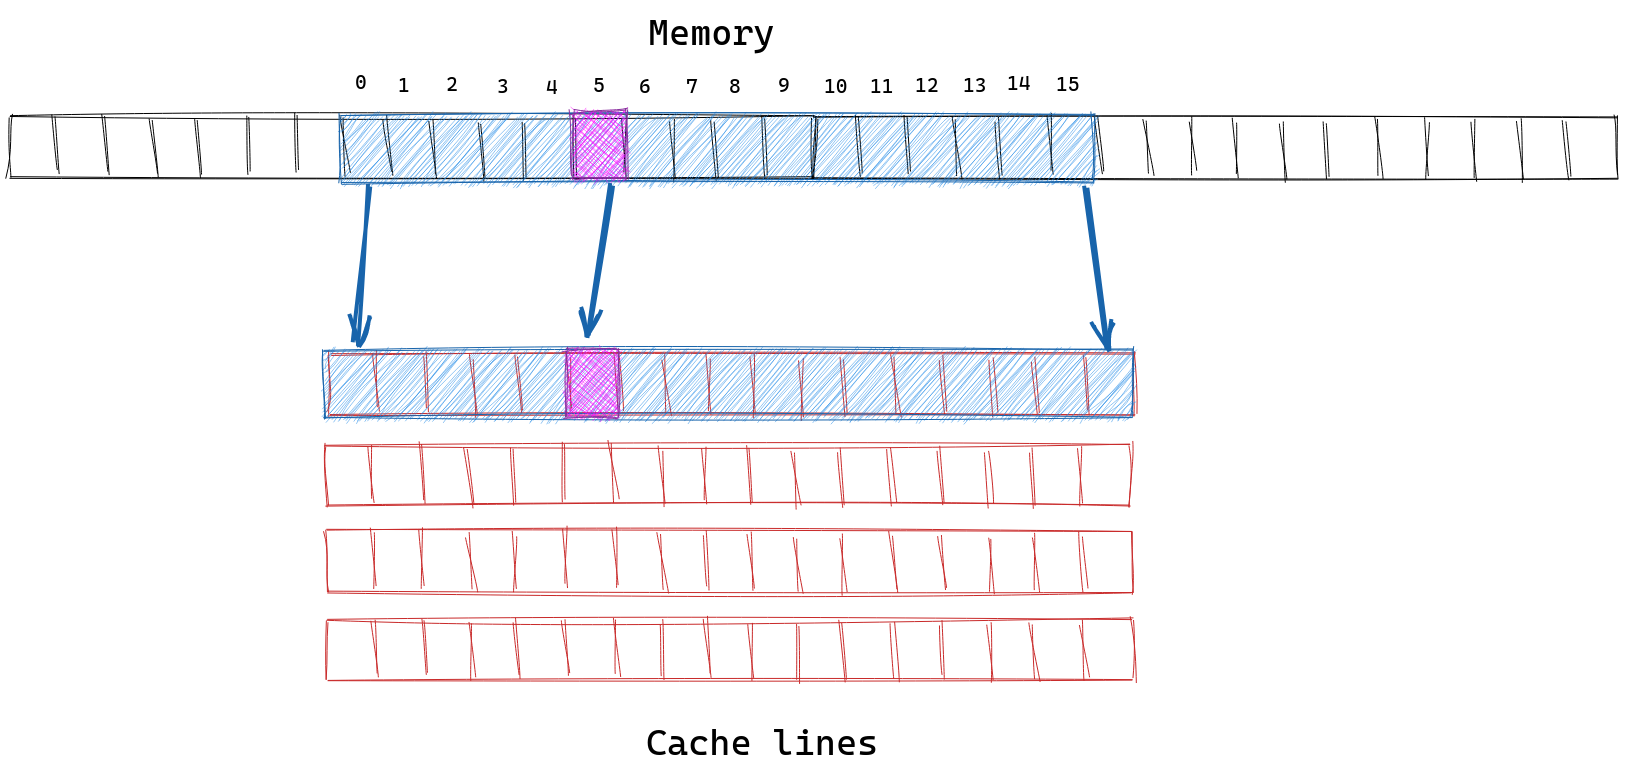
\includegraphics[scale=0.2]{cache-line-copy.png}
\end{frame}

\end{document}
